\documentclass{article}
\usepackage[T1]{fontenc}
\usepackage[utf8]{inputenc}
\usepackage[polish]{babel}
\usepackage[margin=0.5in]{geometry}
\usepackage{graphicx}
\graphicspath{ {./gfx/} }


\title{Matowanie Hetmanem}
\author{Bartłomiej Meller\and Paweł Chłąd}
\date{\today}
\usepackage{hyperref}
\begin{document}

\maketitle


\section{Założenia}
Założeniem Programu jest znajdywanie mata w jednym ruchu dla dwóch króli i hetmana obecnego na szachownicy.


\section{Instrukcja obsługi}

Importujemy moduł klasę "Board"

\begin{center}
    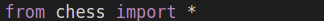
\includegraphics{1}
\end{center}

Tworzymy obiekt szachownicy

\begin{center}
    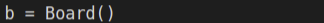
\includegraphics{2}
\end{center}


Ustawiamy figury (figura, pole)

\begin{center}
    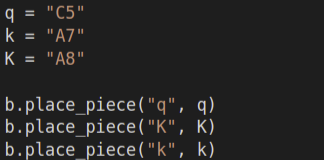
\includegraphics{3}
\end{center}


Sprawdzamy ruchy matujące (figura matująca, matowany król)

\begin{center}
    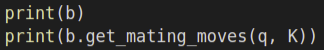
\includegraphics{4}
\end{center}


Wypisujemy szachownicę i listę ruchów matujących

\section{Stos Technologiczny}

\begin{itemize}

\item{Python3.9}

\end{itemize}

\end{document}
